\input{../latex_main/main.tex}

\newcommand{\inducer}{\mathcal{I}}
\newcommand{\R}{\mathds{R}}

%The following might look confusing but allows us to switch the notation of the optimization problem independently from the notation of the hyper parameter optimization
\newcommand{\xx}{\conf} %x of the optimizer
\newcommand{\xxi}[1][i]{\conf_{#1}} %i-th component of xx (not confuse with i-th individual)
\newcommand{\XX}{\pcs} %search space / domain of f
\newcommand{\f}{\cost} %objective function

\newenvironment{blocki}[1] % itemize block
{
 \begin{block}{#1}\begin{itemize}
}
{
\end{itemize}\end{block}
}

\title[AutoML: Hyperparameter Optimization]{AutoML: Hyperparameter Optimization}
%\subtitle{Overview for this Week} %To be defined in source!
%TODO: change authors!
\author[Marius Lindauer]{\underline{Bernd Bischl} \and Frank Hutter \and Lars Kotthoff\newline \and Marius Lindauer \and Joaquin Vanschoren}
\institute{}
\date{}

\subtitle{Grid and Random Search}


\begin{document}

\maketitle


%----------------------------------------------------------------------
%----------------------------------------------------------------------


\begin{frame}[containsverbatim,allowframebreaks]{Grid search}

\begin{columns}
\begin{column}{0.49\textwidth}
\begin{itemize}
\item Simple technique which is still quite popular, tries all
HP combinations on a multi-dimensional discretized grid
\item For each hyperparameter a finite set of candidates is predefined
\item Then, we simply search all possible combinations in arbitrary order
\end{itemize}
\end{column}
\begin{column}{0.49\textwidth}
\vspace*{-0.8cm}
\begin{center}
\begin{figure}
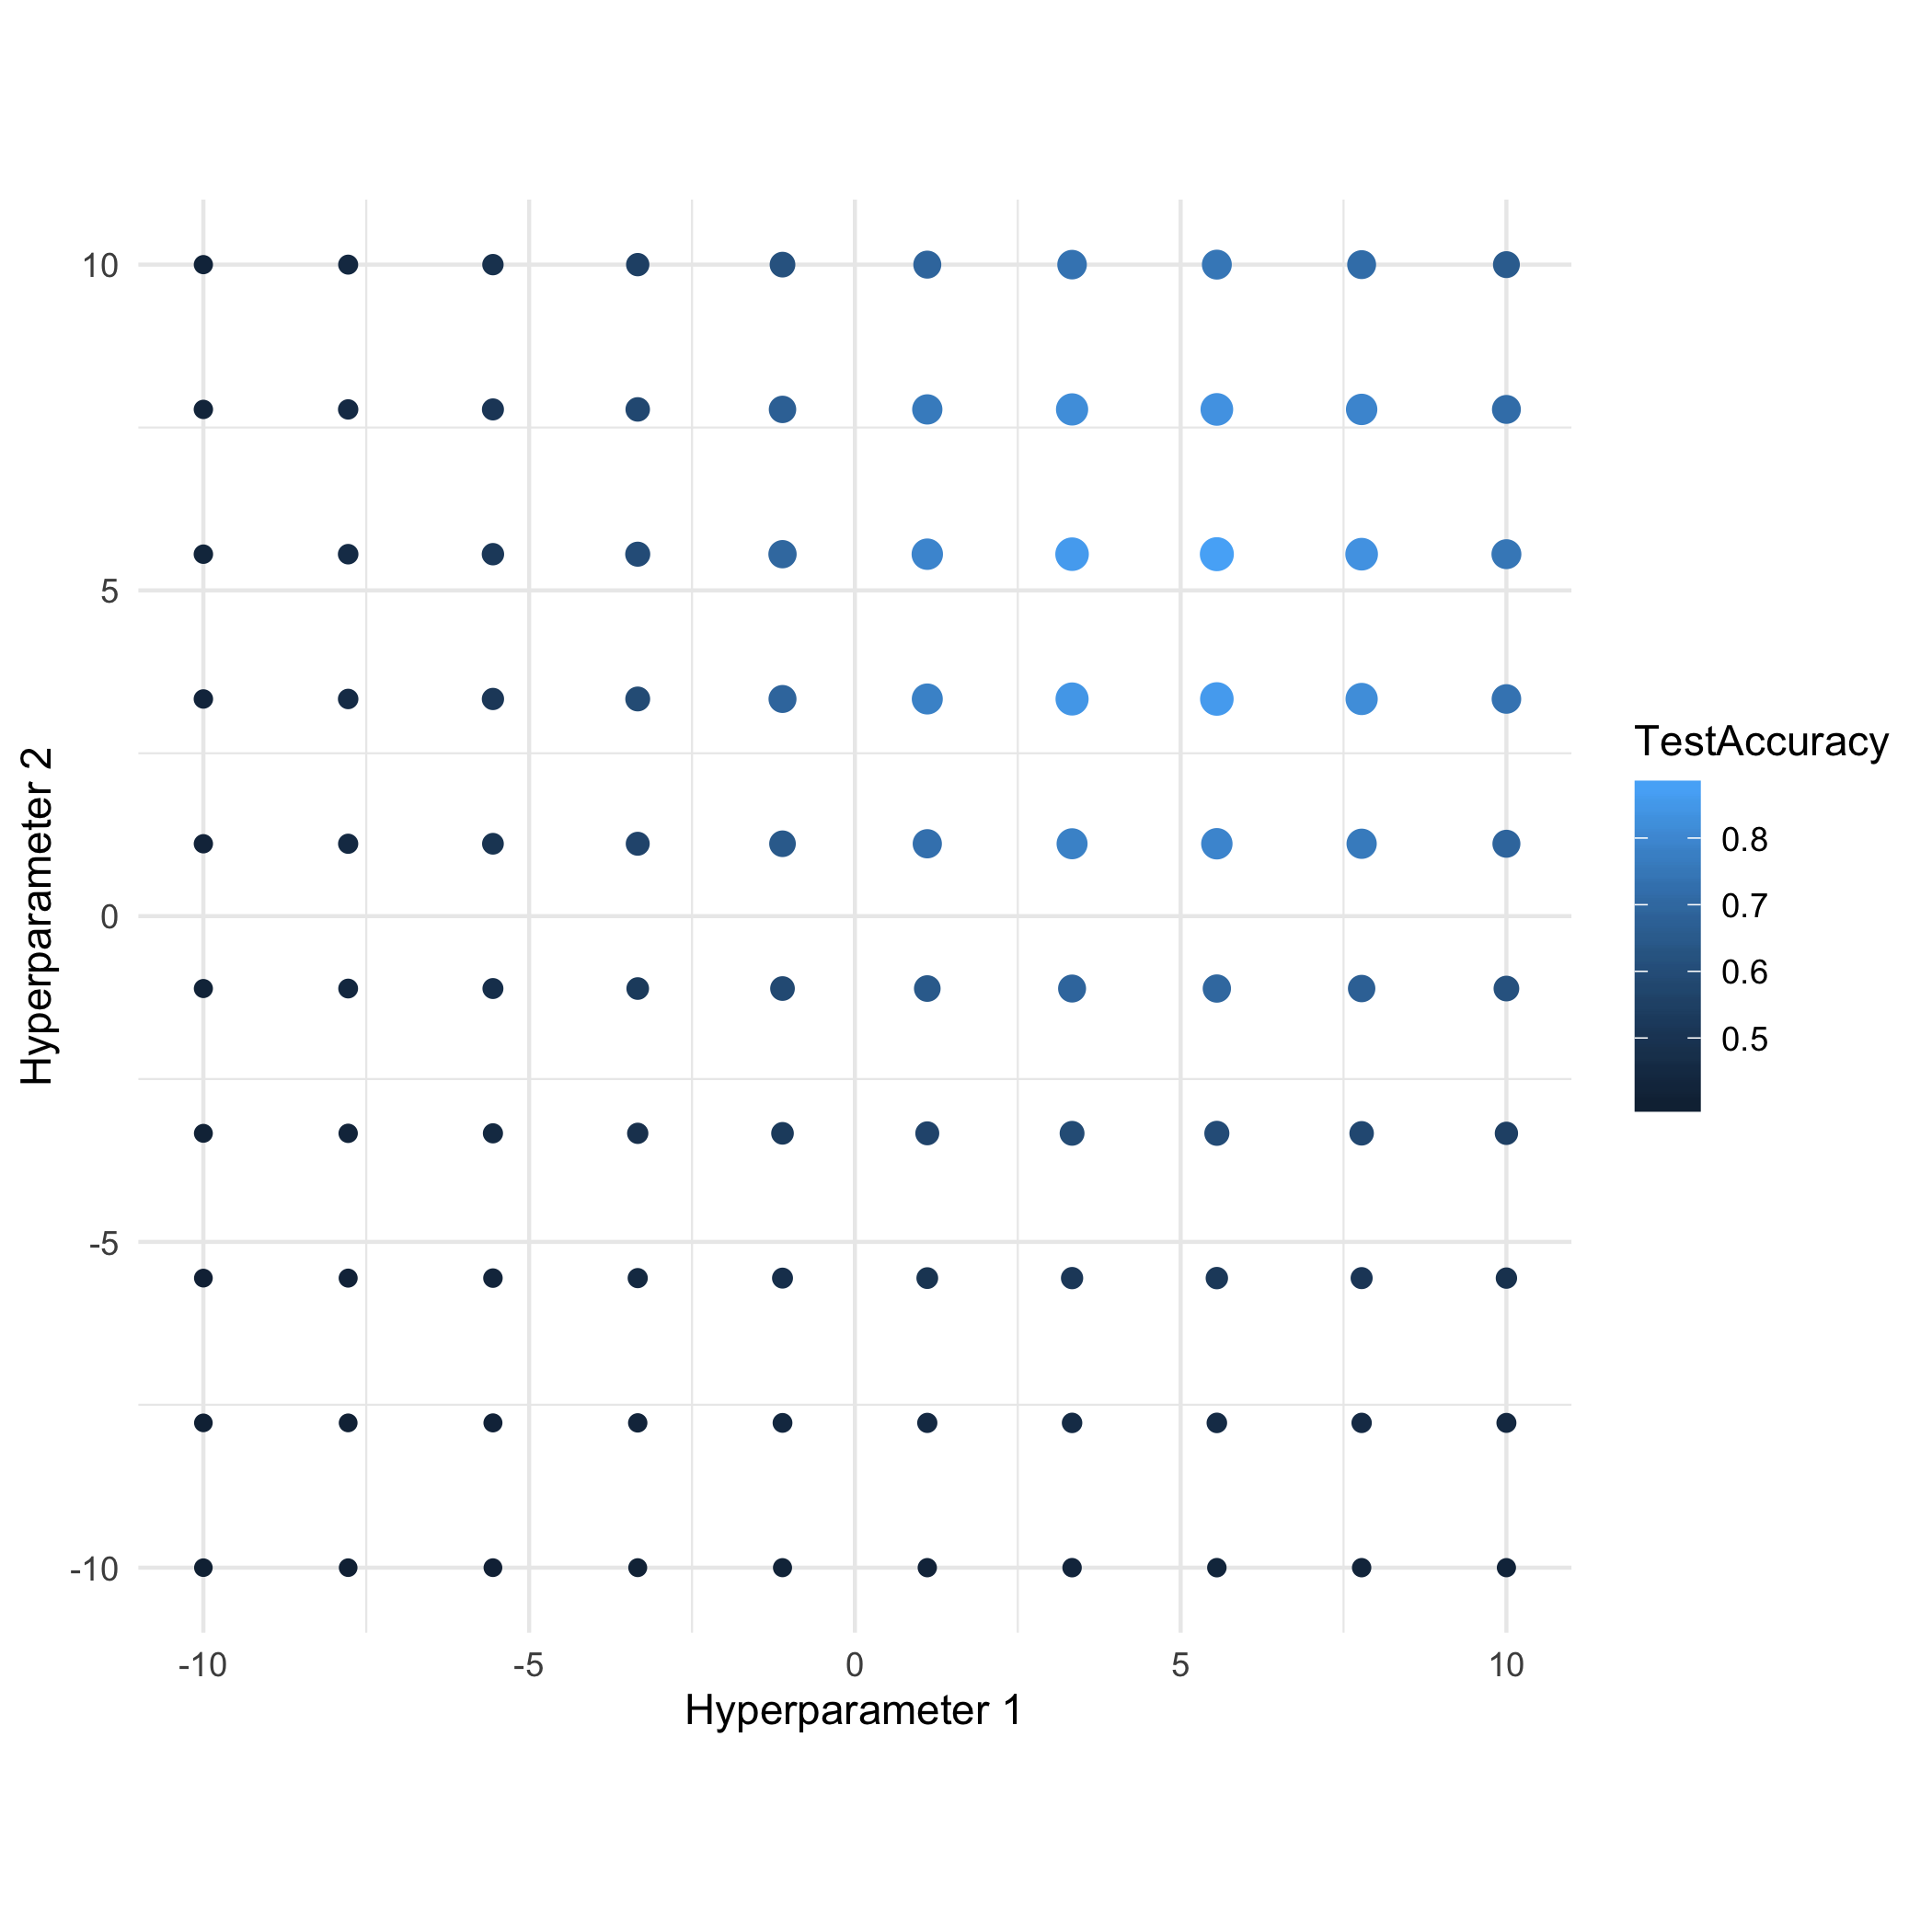
\includegraphics[width=0.9\textwidth]{images/grid.png}
\caption*{Grid search over 10x10 points}
\end{figure}
\end{center}
\end{column}
\end{columns}

\framebreak

\begin{blocki}{Advantages}
\item Very easy to implement
\item All parameter types possible
\item Parallelizing computation is trivial
\end{blocki}

\begin{blocki}{Disadvantages}
\item Scales badly: Combinatorial explosion
\item Inefficient: Searches large irrelevant areas
\item Low resolution in each dimension
\item Arbitrary: Which values / discretization?
\end{blocki}
\end{frame}


\begin{frame}[containsverbatim,allowframebreaks]{Random search}



\begin{columns}
\begin{column}{0.49\textwidth}
\begin{itemize}
\item Small variation of grid search
\item Uniformly sample from the region-of-interest
\end{itemize}
\end{column}
\begin{column}{0.49\textwidth}
\vspace*{-0.8cm}
\begin{center}
\begin{figure}
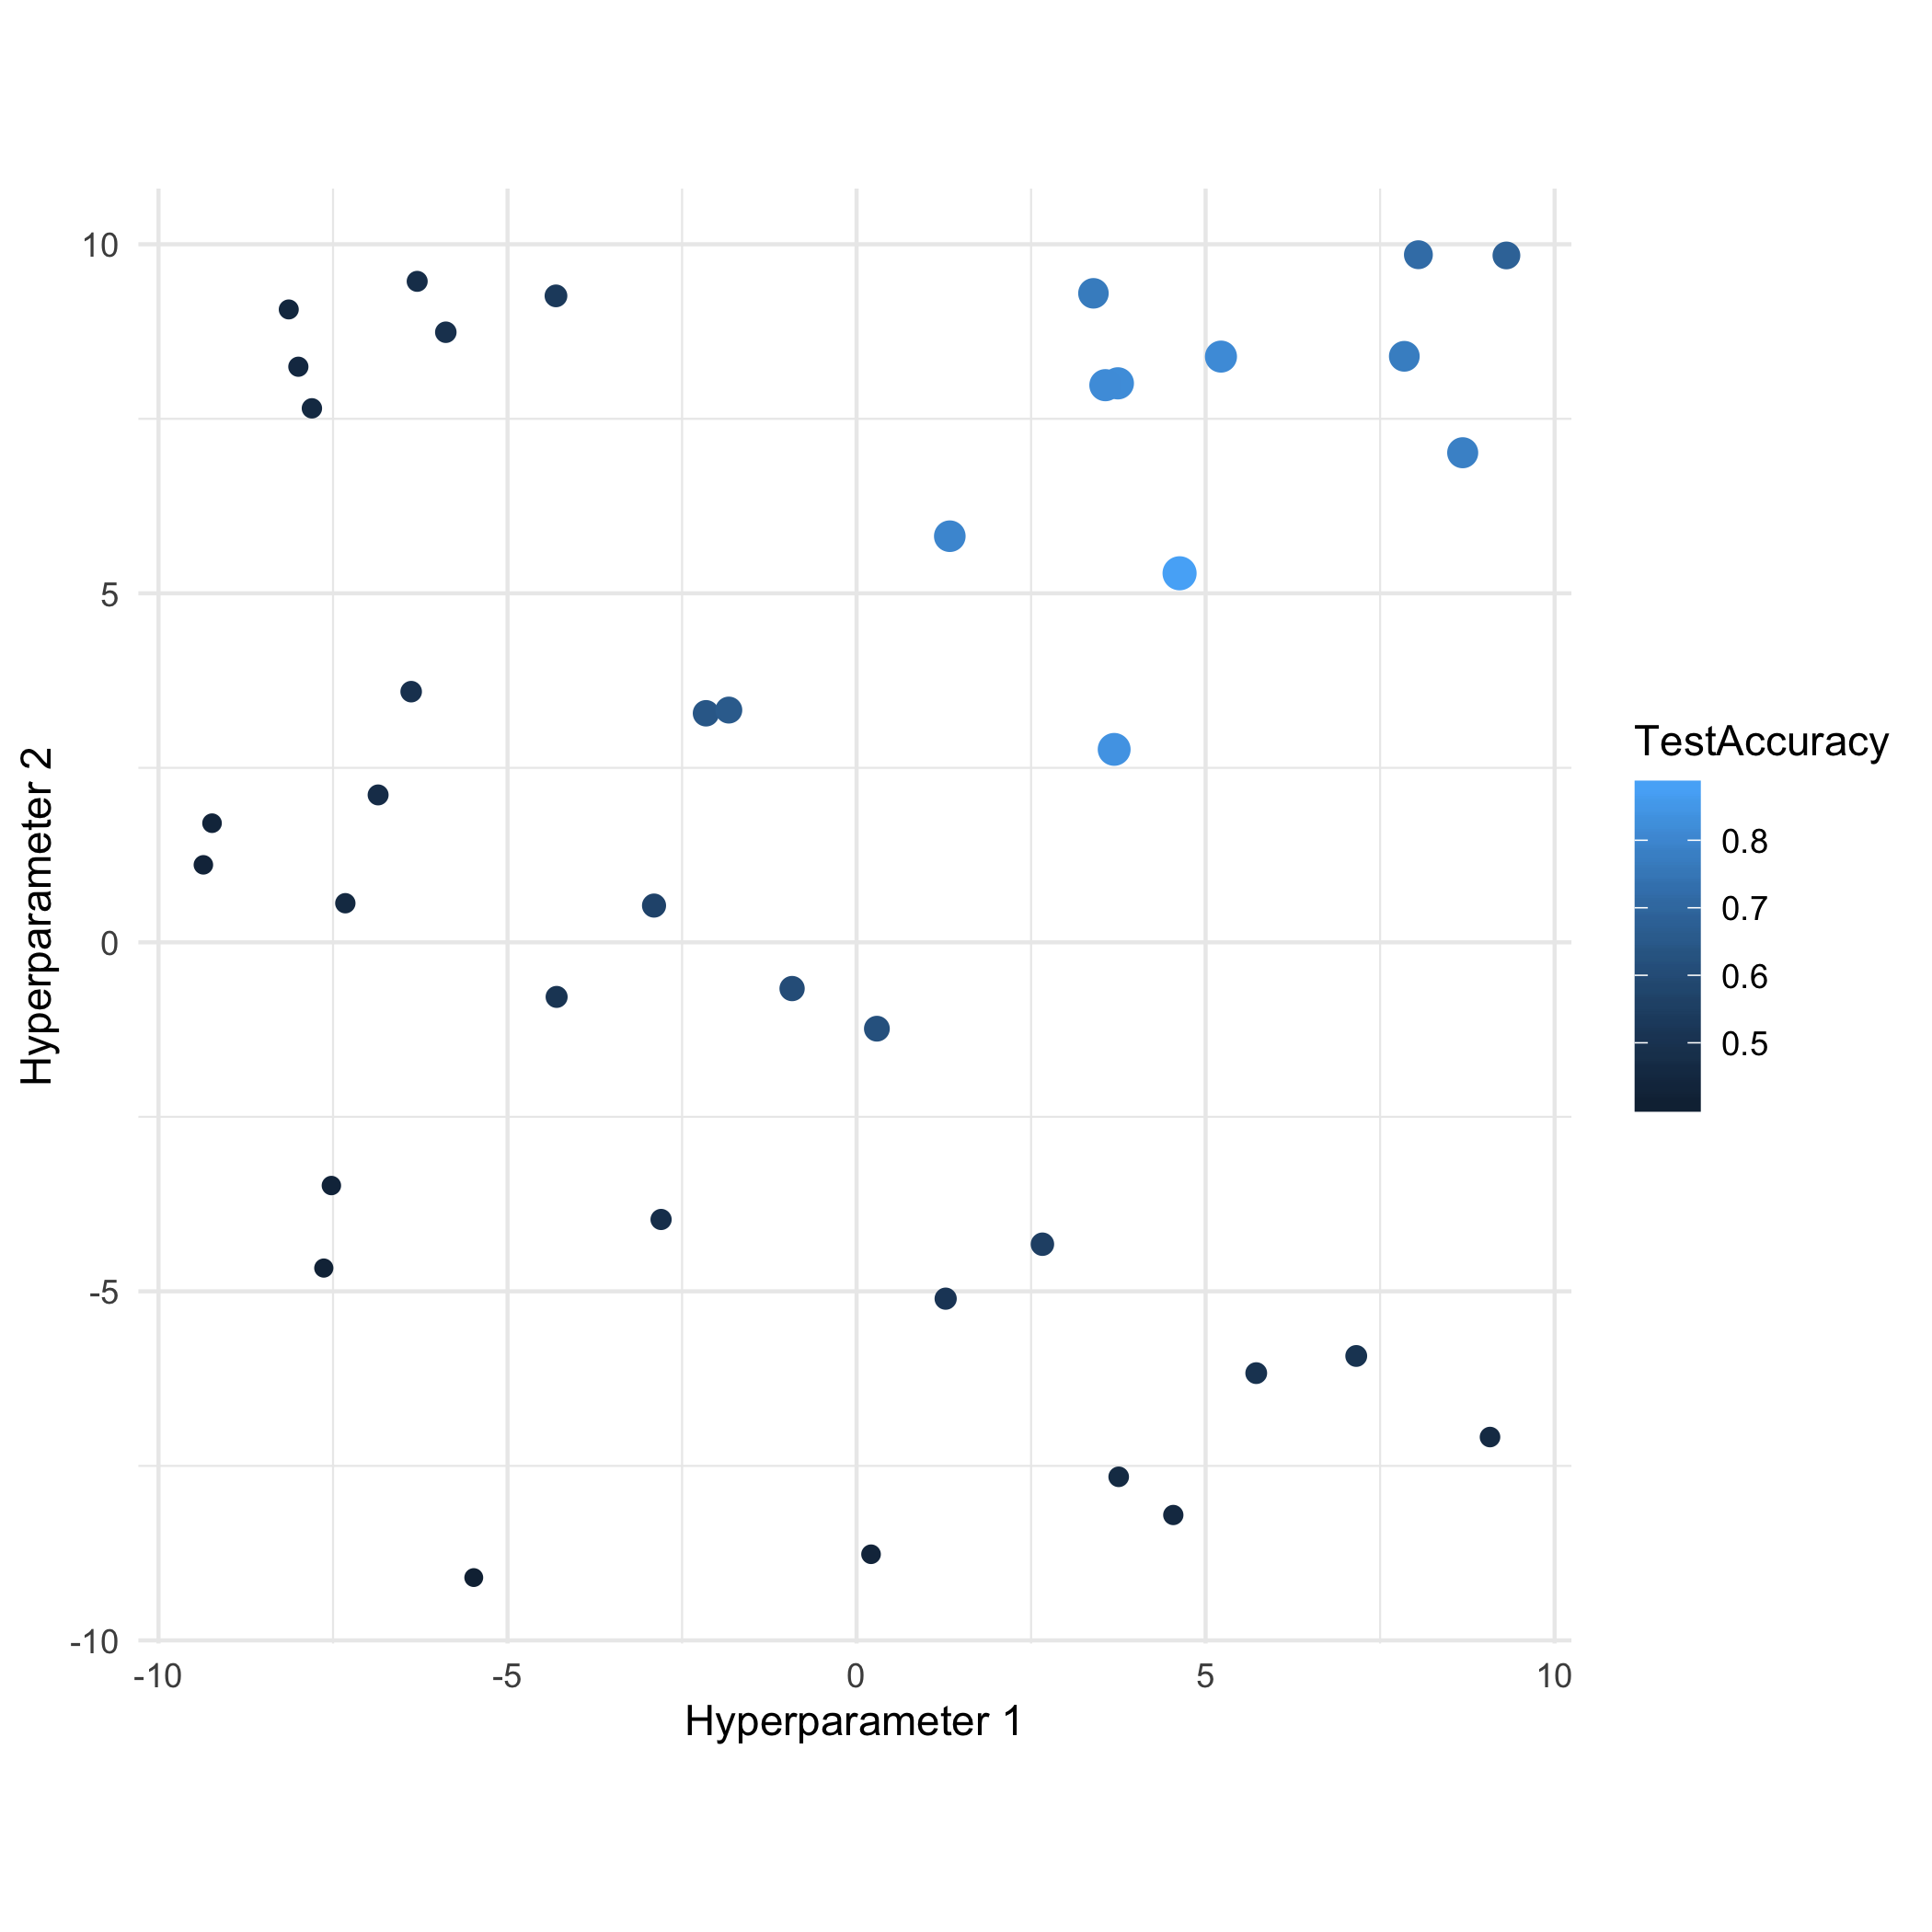
\includegraphics[width=0.9\textwidth]{images/random.png}
\caption*{Random search over 100 points}
\end{figure}
\end{center}
\end{column}
\end{columns}

\framebreak

\begin{blocki}{Advantages}
\item Like grid search: Very easy to implement, all parameter types possible, trivial parallelization
\item Anytime algorithm: Can stop the search whenever our budget for computation is exhausted, or continue until we reach our performance goal.
\item No discretization: each individual parameter is tried with a different value every time
\end{blocki}

\begin{blocki}{Disadvantages}
\item Inefficient: many evaluations in areas with low likelihood for improvement
\item Scales badly: high dimensional hyperparameter spaces need \emph{lots} of samples to cover.
\end{blocki}
\end{frame}

\begin{frame}{Grid search vs. Random search}

\begin{columns}
\begin{column}{0.49\textwidth}
\begin{itemize}
    \item With a tuning budget of $T$ only $T^{\frac{1}{d}}$ unique hyperparmeter values are explored for each $\conf_1, \dots, \conf_d$ in a grid search.
    \item Random search will (most likely) see $T$ different values for each hyperparameter.
    \item Grid search can be disadvantageous if some hyperparameters have little or no influence on the model.
\end{itemize}
\end{column}
\begin{column}{0.49\textwidth}
\vspace*{-0.8cm}
\begin{center}
\begin{figure}
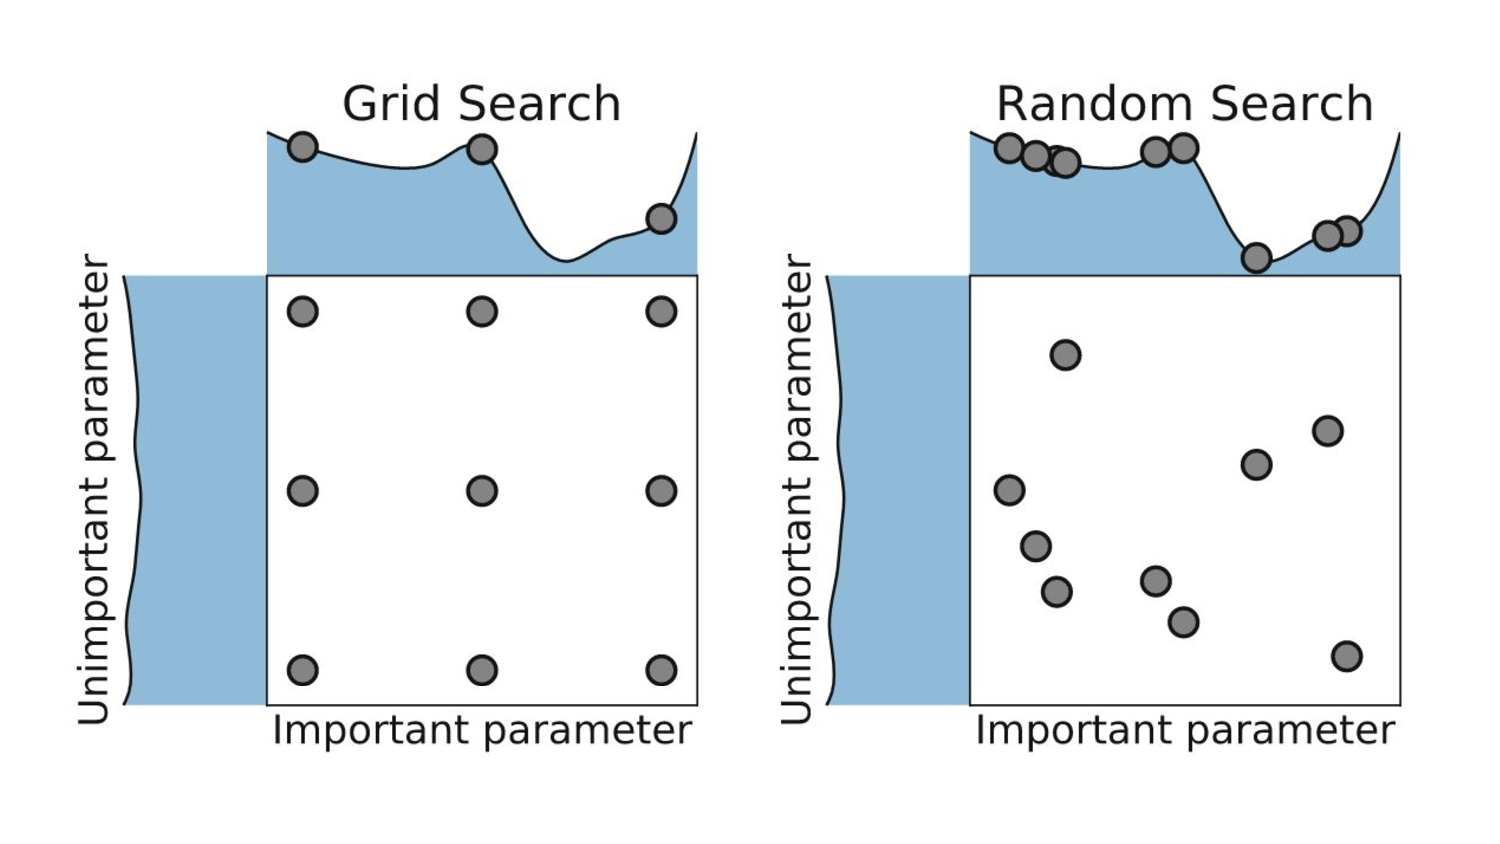
\includegraphics[width=0.9\textwidth]{images/rsvsgs.pdf}
    \caption*{Comparison of grid search and random search. \lit{\href{https://www.automl.org/wp-content/uploads/2019/05/AutoML\_Book.pdf}{Hutter et al. 2019}}}
\end{figure}
\end{center}
\end{column}
\end{columns}

\end{frame}

\end{document}
